\chapter{\selectlanguage{greek}Θεωρητικό Υπόβαθρο}

Στο κεφάλαιο αυτό παρουσιάζονται αρχικά κάποια στοιχεία της θεωρίας γραφημάτων. Έπειτα δίνονται 
κάποια βασικά στοιχεία σχετικά με τη μηχανική μαθηση και ειδικότερα για τα παρακλάδια αυτής
που χρησιμοποιήθηκαν.

\section{Βασικά στοιχεία θεωρίας γραφημάτων}
\subsection{Βασικοί ορισμοί}

Στην Θεωρία  Γραφημάτων ή Γράφων (\en{Graph Theory}), ένας γράφος \(G = (V,E)\)  είναι δομή δεδομένων που
αποτελείται από ένα σύνολο κόμβων \(V\)(\en{nodes}) και ακμών \(E\) (\en{edges}), που 
συνδέουν τους κόμβους μεταξύ τους \cite{Diestel} \cite{barabasi}. Συνήθως ένας γράφος
αναπαρίσταται ως τελείες που συμβολίζουν τους κόμβους και γραμμές μεταξύ των τελειών που
συμβολίζουν τις ακμές. Η σειρά που αναπαριστώνται οι γραμμές και οι τελείες δεν έχει σημασία,
αφού οι γράφοι διατηρούν την πληροφορία τους στον τρόπο με τον οποίο είναι συνδεδεμένοι οι 
κόμβοι μεταξύ τους.

\begin{figure}[!ht] \centering
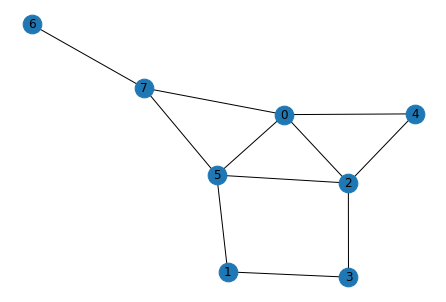
\includegraphics[scale = 0.5]{static/figures/graph_example.png} 
\caption{Παράδειγμα γράφου}
\label{figure1.1}
\end{figure}

Οι γράφοι αποτελούν μια μη-ευκλείδια δομή δεδομένων, που σημαίνει ότι διαφέρουν από
τις παραδοσιακές δομές δεδομένων δύο διαστάσεων, όπως οι εικόνες, ο ήχος και το κείμενο. Οι
κόμβοι αποτελούν οντότητες που συγκρατούν την πληροφορία για κάποιο στοιχείο, ενώ οι ακμές
αντιπροσωπεύουν τη σύνδεση μεταξύ των κόμβων, και μπορούν και αυτές να περιέχουν κάποια
πληροφορία για τη σύνδεση αυτή. Τέλος, οι γράφοι μπορούν να έχουν κάποια χαρακτηριστικά που
ρυθμίζουν τις ενέργειες και την ανάλυση που μπορούμε να εκτελέσουμε πάνω σε αυτούς.

Οι κόμβοι και οι ακμές μπορούν να αποτελούνται από διάφορα στοιχεία:
\begin{itemize}
    \item Είδος (\en{Type})
    \item Ετικέτες (\en{Labels})
    \item Χαρακτηριστικά (\en{Features} (μετάφραση (μτφ.) Γνωρίσματα)/\en{Attributes} (μτφ. Χαρακτηριστικά)
\end{itemize}

Το είδος ενός κόμβου αντιπροσωπεύει την κατηγορία στην οποία εμπίπτει (π.χ. αν αντιπροσωπεύει
άνθρωπο ή κάποιο ζώο). Οι ετικέτες και τα χαρακτηριστικά αποτελούν 2 διαφορετικά στοιχεία,
τα οποία μπορούν να γίνουν διαισθητικά αντιληπτά με το εξής παράδειγμα: εάν ένας κόμβος
συμβολίζει έναν άνθρωπο, τότε η ετικέτα του κόμβου είναι το όνομά του, και τα χαρακτηριστικά
του είναι τα γνωρίσματα που χαρακτηρίζουν το άτομο αυτό (ηλικία, φύλο, εκπαίδευση, κ.λπ.).
Συνήθως στα υπολογιστικά συστήματα για ευκολία ο κάθε κόμβος έχει το δικό του αριθμό
ταυτοποίησης (\en{id}).

Οι ακμές μπορούν να έχουν και αυτές χαρακτηριστικά και ετικέτες (βάρη). Να σημειωθεί εδώ πως
οι ετικέτες και τα χαρακτηριστικά δεν είναι απαραίτητα δεδομένα σε αριθμητική μορφή, αλλά
μπορούν να έχουν και τη μορφή κειμένου.

\subsection{Είδη γράφων} \label{Είδη γράφων}

Στα πλαίσια της παρούσας εργασίας, ένας γράφος \(G\) αποτελείται από μία συνάρτηση χαρτογράφησης ειδών κόμβου \(f_u: V 
\rightarrow T^u\) και αντίστοιχα μια συνάρτηση χαρτογράφησης τύπων ακμών \(F_e: E \rightarrow
T^e\), όπου \(T_u\) και \(T_e\) το σύνολο των ειδών κόμβων και ακμών αντίστοιχα. 

Με βάση τα παραπάνω, οι γράφοι χωρίζονται σε διάφορες κατηγορίες, ανάλογα με το είδος των ακμών και τον κόμβων που τους απαρτίζουν:
\begin{itemize}
    \item \textbf{Ομογενείς}, όταν \(|T^u| = |T^e| = 1\), δηλαδή όλοι ο κόμβοι και οι ακμές 
    είναι ενός τύπου
    \item \textbf{Ετερογενείς}, όταν \(|T^u|>1\) ή/και \(|T^e|>1\), δηλαδή οι κόμβοι ή/και 
    οι ακμές είναι διαφόρων τύπων.
\end{itemize}

Ακόμα, οι γράφοι μπορούν να χαρακτηριστούν ανάλογα με το είδος των ακμών:
\begin{itemize}
    \item \textbf{Μη-κατευθυνόμενοι} (\en{Undirected}), όταν η σύνδεση 2 κόμβων είναι
    αμφίδορμη, δηλαδή μπορεί κανείς να μετακινηθεί από τον κόμβο \(u_a\) στον κόμβο \(u_b\)
    και αντίστροφα μέσω της ίδιας ακμής (\(u_a \leftrightarrow u_b\))
    \item \textbf{Κατευθυνόμενοι} (\en{Directed}), όταν η σύνδεση είναι από τον κόμβο \(u_a\)
    στον κόμβο \(u_b\) προϋποθέτει ακμή αυστηρά από τον κόμβο \(u_a\) προς τον κόμβο \(u_b\)
    (\(u_a \rightarrow u_b\))
\end{itemize}

Επίσης οι γράφοι μπορούν να είναι:
\begin{itemize}
    \item \textbf{Στατικοί}, όταν οι κόμβοι και οι ακμές δεν αλλάζουν 
    π.χ. με την πάροδο του χρόνου 
    \item \textbf{Δυναμικοί}, όταν οι κόμβοι και οι ακμές μπορούν να αλλάξουν, 
    να μετακινηθούν κλπ.
\end{itemize}

Τέλος, ένα \emph{μονοπάτι (\en{path)}} σε ένα γράφο μπορεί να οριστεί ως εξής
\cite{Diestel}: \(P = (V,E)\) όπου \(V =\{x_0,x_1,\cdots,x_k\}\) και
\(E = \{(x_0,x_1),(x_1,x_2),\cdots,(x_{k-1},x_k)\}\), όπου \(V \subseteq V_G\) και \(E 
\subseteq E_G\). Ένας \emph{περίπατος} (\en{walk}) μπορεί να ειδωθεί σαν ένα μονοπάτι  στο οποίο κορυφές ή/και ακμές μπορουν να επαναληφθούν. \emph{Μήκος μονοπατιού/περιπάτου} είναι ο αριθμός των ακμών που περιέχει το μονοπάτι ή ο περίπατος. 

\section{Επιστήμη δικτύων}

Η επιστήμη δικτύων και η θεωρία γράφων είναι δύο βαθιά συσχετιζόμενα επιστημονικά πεδία,
τα οποία ωστόσο έχουν κάποιες διαφορές. Η θεωρία γράφων ασχολείται με τη μαθηματική ανάλυση και παρέχει ένα πλήθος αλγορίθμων
που μπορούν να εφαρμοστούν σε όλους τους γράφους, ανεξαρτήτως του προβλήματος που 
αντιπροσωπεύουν. Η επιστήμη δικτύων εστιάζει σε προβλήματα που βρίσκονται στον πραγματικό
κόσμο. Ο γράφος μετονομάζεται σε δίκτυο, και αναλύονται δίκτυα μεταφορών, κοινωνικά δίκτυα
κ.λπ. Η επιστήμη δικτύων  αναπτύχθηκε παράλληλα  με την των υπολογιστικών συστημάτων.

\subsection{Μετρικές ομοιότητας}

Στην επιστήμη δικτύων μελετάται η δομή και τα χαρακτηριστικά ενός δικτύου με σκοπό την 
εξαγωγή πληροφορίας και συμπερασμάτων για την επίλυση ενός προβλήματος. Για το σκοπό αυτό
έχουν αναπτυχθεί μετρικές ομοιότητας οι οποίες ποσοτικοποιούν την ομοιότητα μεταξύ των 
κόμβων. Αυτή η ανάλυση είναι χρήσιμη διότι σε πολλά προβλήματα στην επιστήμη δικτύων,
σημαντικό μέρος της λύσης αποτελεί η εύρεση ````γειτονιών'''', δηλαδή ομάδων κόμβων με κοινά
χαρακτηριστικά και γειτονικούς κόμβους, ή η εύρεση ````όμοιων'''' κόμβων σύμφωνα με κάποιες μετρικές.
Στη συνέχεια θα παρουσιαστούν ορισμένες από αυτές, οι οποίες είναι σχεδιασμένες έτσι ώστε
με δεδομένους 2 κόμβους, μια μετρική να δίνει υψηλότερη τιμή αν οι 2 κόμβοι είναι ````όμοιοι''''.

\subsubsection{Απόσταση}

Η Απόσταση (\en{Graph Distance}) εκφράζει την απόσταση μεταξύ 2 κόμβων \(x,y\) μέσα σε ένα δίκτυο.
Ορίζεται ως το μήκος του μικρότερου μονοπατιού οπό τον κόμβο
    $x$ στον κόμβο $y$ και συμβολίζεται ως $GD(x,y)$.

Για την εύρεση της απόστασης είναι υποβέλτιστο να εφαρμοστεί ο αλγόριθμος του 
\en{Dijkstra} \cite{Dijkstra1959}.
Αντί για αυτό, δημιουργούνται και αρχικοποιούνται 2 σύνολα κόμβων \(S = \{x\}\) 
και \(D = \{y\}\). Με κάθε επανάληψη, προστίθενται σε κάθε σύνολο εναλλάξ οι γείτονες των 
κόμβων του κάθε συνόλου. Με τον όρο γείτονες εννοούμε τους κόμβους 
που έχουν ακμή με τους
κόμβους που ανήκουν σε κάθε σύνολο και δεν είναι ηδη σε αυτά. Η διαδικασία τερματίζεται 
όταν
\(S \cap D \neq 0\). Η τιμή της απόστασης είναι ο αριθμός των βημάτων που απαιτήθηκαν. Το
αρνητικό πρόσημο εισάγεται για να ικανοποιήσει τον περιορισμό πως η τιμή αυξάνει όσο οι 
κόμβοι \(x,y\) πλησιάζουν \cite{GraphDistance}.

\subsection{Κοινοί γείτονες}

Οι κοινοί γείτονες (\en{Common neighbours}) εκφράζει την έννοια πως όσο περισσότερους κοινούς
γείτονες έχουν 2 κόμβοι, τόσο πιο ````όμοιοι'''' είναι. Ορίζεται ως
 \begin{equation}
     CN(x,y) = |\Gamma(x)\cap\Gamma(y)|
 \end{equation}

οπου \(\Gamma(x)\) το σύνολο των γειτόνων του κόμβου \(x\) \cite{CN}.

\subsection{Συντελεστής \en{Jaccard}}

Ο συντελεστής \en{Jaccard} εκφράζει την πιθανότητα οι κόμβοι \(x,y\) να έχουν κάποιο κοινό
γείτονα. Ορίζεται ως:

\begin{equation}
    Jaccard(x,y) = \frac{|\Gamma(x)\cap\Gamma(y)|}{|\Gamma(x)\cup\Gamma(y)|}
\end{equation}

Συγκρινόμενη με την μετρική κοινών γειτόνων (\en{CN}) ο συντελεστής \en{Jaccard} εξαλείφει
την πιθανότητα οι κόμβοι \(x,y\) να έχουν κοινούς γείτονες, επειδή έχουν πολλούς γείτονες
\cite{kosub2016note}.

\subsection{Συντελεστής \en{Adamic/Adar}}

Ο συντελεστής \en{Adamic/Adar} εκφράζει την ιδιότητα των κοινών γειτόνων με τη διαφορά 
ότι ευνοεί τις περιπτώσεις που κόμβοι έχουν λίγους γείτονες. Όταν ένας κόμβος έχει μικρό
αριθμό γειτόνων, τότε η σημασία κάθε ακμής (συσχέτισης με άλλο κόμβο) είναι υψηλότερη 
σε σχέση με το αν είχε περισσότερους γείτονες\cite{Adamic2003FriendsAN}. Ορίζεται ως:

\begin{equation}
    AA(x,y) = \sum_{z \in \Gamma(x)\cap\Gamma(y)} \frac{1}{\log|\Gamma(z)|}
\end{equation}

\subsection{Άλλες μετρικές}

Υπάρχουν ακόμα πολλές μετρικές ομοιότητας, ακόμη και ολόκληροι αλγόριθμοι όπως ο 
\en{PageRank} της \en{Google} \cite{ilprints422}. O συγκεκριμένος αλγόριθμος βασίζεται 
στην ιδέα πως όσο περισσότερες ακμές καταλήγουν σε έναν κόμβο (για κατευθυνόμενους γράφους)
τόσο σημαντικότερος είναι ο κόμβος αυτός. Επίσης, η μετρική \en{Katz} είναι μια παραλλαγή
της απόστασης (\en{GD}) και εκφράζει την ιδέα πως όσο περισσότερα μονοπάτια υπάρχουν
μεταξύ 2 κόμβων και όσο μικρότερα είναι αυτά, τόσο πιο όμοιοι είναι αυτοί οι κόμβοι 
\cite{RePEc:spr:psycho:v:18:y:1953:i:1:p:39-43}:

\begin{equation}
    Katz(x,y) = \sum_{l=1}^{\infty} \beta^l\dot|Path_{x,y}^l|
\end{equation}

όπου \(l\) το μήκος μονοπατιού και \(\beta\) ο συντελεστής απόσβεσης ανάλογα με το μήκος.

\section{Τα δίκτυα στα υπολογιστικά συστήματα}

Πως όμως αποθηκεύεται ένα δίκτυο σε ένα υπολογιστικό σύστημα? Μια πρώτη σκέψη θα ήταν να
αποθηκευτεί ο πίνακας γειτνίασης του γράφου \(A\), ο οποίος είναι διαστάσεων 
\(N \times N ,N = |V|\), όπου 
\begin{equation}
    A_{ij} = 
    \begin{cases}
        w_{ij} & \text{αν} (u_i,u_j) \in E \\
        0 & \text{αλλιώς}
    \end{cases}
\end{equation}

όπου \(w_{ij}\) το βάρος (αν υπάρχει, αλλιώς 1) της ακμής μεταξύ των κόμβων \(u_i\) και
\(u_j\). 

Από αυτή τη σκέψη προκύπτουν δύο μεγάλα προβλήματα. Αρχικά, γίνεται εύκολα αντιληπτό πως ο
πίνακας \(A\) γίνεται τεράστιος όσο αυξάνονται τα δεδομένα, και έπειτα δεν αποθηκεύεται
κάποια άλλη πληροφορία για τους κόμβους ή τις ακμές. Έχει επικρατήσει λοιπόν στην
επιστημονική κοινότητα οι γράφοι να αποθηκεύονται ως μια λίστα ακμών (\en{edgelist}) όπου
στην πρώτη και δεύτερη στήλη αποθηκεύονται ο αρχικός και τελικός κόμβος της ακμής, στην
τρίτη το βάρος της ακμής και σε κάθε επόμενη στήλη οποιοδήποτε άλλο χαρακτηριστικό της
ακμής, αν υπάρχει. Οι κόμβοι προκύπτουν από τη λίστα αυτή, ή
αν έχουν χαρακτηριστικά τότε αυτά αποθηκεύονται ως πίνακας \(N \times K\) όπου \(N\) ο
αριθμός των κόμβων και \(K\) το πλήθος των χαρακτηριστικών για κάθε κόμβο. Για τον εύκολο
χειρισμό αυτών των δομών δεδομένων έχουν αναπτυχθεί ειδικά πακέτα λογισμικού για αυτό το σκοπό(π.χ. 
\cite{StellarGraph}, \cite{Networkx}).

\section{Μηχανική μάθηση}

\subsection{Γενικά για τη μηχανική μάθηση}

Η μηχανική μάθηση αποτελεί υποσύνολο της επιστήμης της τεχνητής νοημοσύνης. Η γενική
αρχή της μηχανικής μάθησης είναι ότι χρησιμοποιούνται αλγόριθμοι για την επίλυση ενός 
προβλήματος, οι οποίοι έχουν την ιδιότητα να βελτιώνουν την ορθότητα της λύσης τους
μέσω μιας διαδικασίας εκπαίδευσης\cite{DataMining}. Για να επιτευχθεί αυτό χρησιμοποιούνται
τα δεδομένα εισόδου του προβλήματος, χωρίς να χρειάζεται η παρέμβαση του προγραμματιστή/αναλυτή.
Η μηχανική μάθηση έχει γνωρίσει  ιδιαίτερα μεγάλη ανάπτυξη τα τελευταία χρόνια και εφαρμόζεται σε
ολοένα και περισσότερα πολύπλοκα προβλήματα σε πολλούς και διαφορετικούς τομείς.

Για την εκπαίδευση του αλγορίθμου, αρκεί να δοθεί ένα σύνολο από δεδομένα εκπαίδευσης.
Χρησιμοποιώντας αυτά, ο αλγόριθμος παράγει ένα σύνολο από κανόνες, διαμορφωμένους από τα
δεδομένα αυτά, δημιουργώντας επι του πρακτέου ένα νέο αλγόριθμο, που στη βιβλιογραφία 
αναφέρεται και ως \emph{Μοντέλο}. Το μοντέλο που θα δημιουργηθεί εξαρτάται άμεσα από τα
δεδομένα εκπαίδευσης. Για παράδειγμα, ο ίδιος αλγόριθμος μπορεί να χρησιμοποιηθεί για
τη δημιουργία ενός μοντέλου μετάφρασης από μια γλώσσα σε μια άλλη, ή για την ανάπτυξη
ενός μοντέλου πρόβλεψης της αγοράς του χρηματιστηρίου.

Είναι λογικό να συμπεράνει κανείς πως όσο περισσότερα δεδομένα εκπαίδευσης δοθούν στον 
αλγόριθμο, τόσο καλύτερο μοντέλο θα παραχθεί. Αυτό φαίνεται και από γεγονός πως το 
επιστημονικό πεδίο της μηχανικής μάθησης αναπτύχθηκε ραγδαία μαζί με την ανάπτυξη του
διαδικτύου, που έδωσε πρόσβαση σε ένα τεράστιο όγκο δεδομένων.

\subsection{Κατηγορίες μηχανικής μάθησης}

Η μηχανική μάθηση χωρίζεται σε πολλές κατηγορίες, σύμφωνα με τον τρόπο εκμάθησης 
του αλγορίθμου από τα δεδομένα, ενώ οι κυριότερες είναι:

\begin{itemize}
    \item \textbf{Επιβλεπόμενη} (\en{Supervised}) μάθηση: Ο αλγόριθμος παίρνει στην είσοδο
    μαζί με τα δεδομένα εκπαίδευσης και την αποζητούμενη έξοδο. Έτσι προσαρμόζει το μοντέλο
    ώστε να βγάζει την επιθυμητή έξοδο για τα δεδομένα εισόδου.
    \item \textbf{Μη-επιβλεπόμενη} (\en{Unsupervised}) μάθηση: Τα δεδομένα εισόδου δεν
    συνοδεύονται από την επιθυμητή έξοδο, και ο αλγόριθμος αναζητά μοτίβα (\en{patterns})
    στα δεδομένα. Για παράδειγμα στο ηλεκτρονικό εμπόριο, μοντέλα ανακαλύπτουν ορισμένα
    προϊόντα συνήθως αγοράζονται μαζί.
    \item \textbf{Ενισχυτική} (\en{Reinforcement})
    μάθηση: Ο αλγόριθμος αλληλοεπιδρά 
    με ένα δυναμικό περιβάλλον και διαμορφώνει το μοντέλο σύμφωνα με μια σειρά κανόνων
    επιβράβευσης και τιμωρίας. Για παράδειγμα ο αλγόριθμος πίσω από ένα 
    αυτοδηγούμενο αυτοκίνητο επιβραβεύεται αν το όχημα παραμένει στον δρόμο.
\end{itemize}


\subsection{Δεδομένα και επεξεργασία} \label{Δεδομένα και επεξεργασία}

Όπως είναι φανερό, η αποτελεσματικότητα των τεχνικών μηχανικής μάθησης εξαρτάται άμεσα
από την ποσότητα και την ποιότητα των δεδομένων που χρησιμοποιούνται. Η συλλογή και η 
επεξεργασία δεδομένων αποτελεί ένα πολύ μεγάλο κεφάλαιο στο πεδίο αυτό, ενώ στα πλαίσια της 
εργασίας αυτής θα μας απασχολήσει το δεύτερο. 

Τα συστήματα μηχανικής μάθησης όπως αναφέρθηκε στην ουσία τους αποτελούν μαθηματικά μοντέλα
και αλγορίθμους και τα δεδομένα τα οποία δύνανται να επεξεργαστούν πρέπει να είναι 
συγκεκριμένης μορφής. Στις τεχνικές που θα χρησιμοποιηθούν στην εργασία αυτή, τα
δεδομένα θα πρέπει να είναι σε μορφή πίνακα \(N \times M\) όπου \(N\) ο το πλήθος των
παρατηρήσεων και \(M\) το πλήθος των μεταβλητών εισόδου για κάθε παρατήρηση. Για παράδειγμα
τα δεδομένα προκύπτουν από την παρατήρηση της ρίψης ζαριών, \(N\) θα είναι οι φορές
που θα ριφθεί το ζάρι, και \(M\) θα είναι ίσο με τον αριθμό των ζαριών που ρίπτονται.
Μια πρώτη πρόκληση λοιπόν που συναντήθηκε είναι η μετατροπή των δεδομένων από μορφή
γράφου σε μορφή πίνακα. 

\section{Γράφοι και μηχανική μάθηση}

Στη βιβλιογραφία υπάρχουν πολλές εφαρμογές τεχνικών μηχανικής μάθησης απευθείας  σε
γράφους \cite{zhang2018deep}. Στα πλαίσια της εργασίας αυτής, όπως αναλύθηκε και διατυπώθηκε
το πρόβλημα, κρίθηκε απαραίτητη η χρήση ενός συστήματος μηχανικής μάθησης που λειτουργεί
με δεδομένα πίνακα, όπως αναφέρθηκε στην Ενότητα \ref{Δεδομένα και επεξεργασία}. Μια 
τέτοια υλοποίηση θα απλοποιούσε το πρόβλημα διευκολύνοντας την επίλυσή του, καθιστώντας
το παράλληλα πιο κατανοητό στον αναγνώστη.

Το πρόβλημα της εκμάθησης αναπαραστάσεων γράφων έχει απασχολήσει στο παρελθόν την
επιστημονική κοινότητα \cite{cai2017comprehensive}. Είναι δυνατόν ένας γράφος να 
αναπαρασταθεί με ποικίλλους τρόπους, ανάλογα με το είδος του γράφου εισόδου και
τις απαιτήσεις κάθε προβλήματος (δείτε Ενότητα \ref{Είδη γράφων}). Ανάμεσα στις δημοφιλέστερες
λύσεις βρίσκεται η χρήση τεχνικών μηχανικής μάθησης για εκμάθηση αναπαραστάσεων 
από γράφους, και ειδικότερα η χρήση βαθιάς μάθησης (\en{Deep Learning}). 

Η βαθιά μάθηση (\en{Deep Learning}) είναι μια οικογένεια τεχνικών μηχανικής μάθησης που
βασίζεται σε τεχνητά νευρωνικά δίκτυα (\en{Artificial Neural Networks - ANN})
(δείτε π.χ. \cite{Schmidhuber2015DeepLI} \cite{Goodfellow2015DeepL}). Το όνομα ````βαθιά'''' δόθηκε
στην συγκεκριμένη οικογένεια αλγορίθμων επειδή τα νευρωνικά δίκτυα που χρησιμοποιούνται
αποτελούνται από πολλά στρώματα τα οποία βελτιστοποιούν την ικανότητά τους να μαθαίνουν.
Στο πρόβλημα της εκμάθησης αναπαραστάσεων γράφων η χρήση βαθιάς μάθησης είναι
ευρέως διαδεδομένη και έχουν αναπτυχθεί 2 οικογένειες τεχνικών για την επίτευξή της:

\begin{itemize}
    \item \textbf{\emph{Με} τυχαίους περίπατους}
    \item \textbf{\emph{Χωρίς} τυχαίους περίπατους}
\end{itemize}

\subsection{Αναπαράσταση με χρήση τυχαίων περιπάτων}

Η αναπαράσταση γράφων με χρήση τυχαίων περιπάτων εμπίπτει στην οικογένεια των 
μη επιβλεπόμενων (\en{Unsupervised}) τεχνικών και βασίζεται στην ιδέα πως για να διατηρηθούν
τα δομικά χαρακτηριστικά ενός γράφου, τότε κόμβοι που βρίσκονται ````κοντά'''' στο γράφο τότε
θα αναπαρασταθούν εξίσου ````κοντά'''' και στο χώρο αναπαράστασης. Για την επίτευξη του σκοπού
αναπτύχθηκε αρχικά η τεχνική \en{DeepWalk} \cite{DeepWalk}. Η τεχνική αυτή υιοθετεί 
ένα μοντέλο νευρωνικών δικτύων, ονόματι \en{SkipGram}.Το μοντέλο αυτό
παρουσιάστηκε για πρώτη φορά στα πλαίσια του \en{Word2Vec} \cite{word2vec}.

\subsubsection{\en{SkipGram}} \label{SkipGram}

Στην παράγραφο αυτή θα δοθεί ο συνοπτικά τρόπος λειτουργίας του μοντέλου \en{SkipGram}. Το
μοντέλο αυτό αναπτύχθηκε στα πλαίσια του \en{Word2Vec}, ενός αλγορίθμου που εξάγει
αναπαραστάσεις για ````λέξεις''''. Δηλαδή, παίρνει σαν είσοδο μια ````λέξη'''' (ένα \en{string}) και το
παραμετροποιεί σε ένα διάνυσμα \(1 \times d\), όπου \(d\) ο αριθμός διαστάσεων που θέλουμε.
Ο σκοπός του αλγορίθμου είναι να αναπαραστήσει λέξεις που εμφανίζονται συχνά ````κοντά'''',
με παρόμοια αναπαράσταση. Για παράδειγμα, η λέξεις ````Σοβιετική'''' και ````Ένωση'''' θα αναπαρασταθούν
πολύ πιο όμοια σε σχέση με τις λέξεις ````μήλο'''' και ````αυτοκίνητο''''.

Για το σκοπό αυτό, εκπαιδεύεται ένα νευρωνικό δίκτυο με ένα κρυφό στρώμα ώστε να εκτελεί
μια συγκεκριμένη εργασία. Ο σκοπός όμως δεν είναι η χρήση του νευρωνικού για την εργασία
αυτή, αλλά η εκμάθηση και εξαγωγή των βαρών του κρυφού στρώματος! Στην πραγματικότητα
αυτά τα βάρη είναι οι αναπαραστάσεις των λέξεων που περιεγράφηκαν παραπάνω.

Το νευρωνικό δίκτυο εκπαιδεύεται για την εξής εργασία: Δεδομένης μιας συγκεκριμένης ````λέξης''''
που βρίσκεται σε μια πρόταση, ελέγχει τις γειτονικές λέξεις και επιλέγει μια
με τυχαίο τρόπο. Το νευρωνικό δίκτυο θα πρέπει να δώσει στην έξοδο την πιθανότητα για
κάθε λέξη από ένα προκαθορισμένο λεξιλόγιο να είναι αυτή η ````τυχαία λέξη''''. Η έξοδος δηλαδή 
θα εκφράζει την πιθανότητα να βρεθεί κάθε λέξη από το λεξιλόγιο κοντά στη λέξη εισόδου.

Η εκπαίδευση του νευρωνικού γίνεται βάζοντας στην είσοδο ζευγάρια λέξεων που βρίσκονται
στα δεδομένα εκπαίδευσης. Στο παρακάτω  Σχήμα (\ref{figure1.2}) φαίνονται μερικά 
δείγματα εκπαίδευσης (ζευγάρια λέξεων). Στο συγκεκριμένο παράδειγμα χρησιμοποιείται ένα μέγεθος 
παραθύρου ίσο με 2. Το μέγεθος του παραθύρου αποτελεί παράμετρο του μοντέλου.

\begin{figure}[!ht] \centering
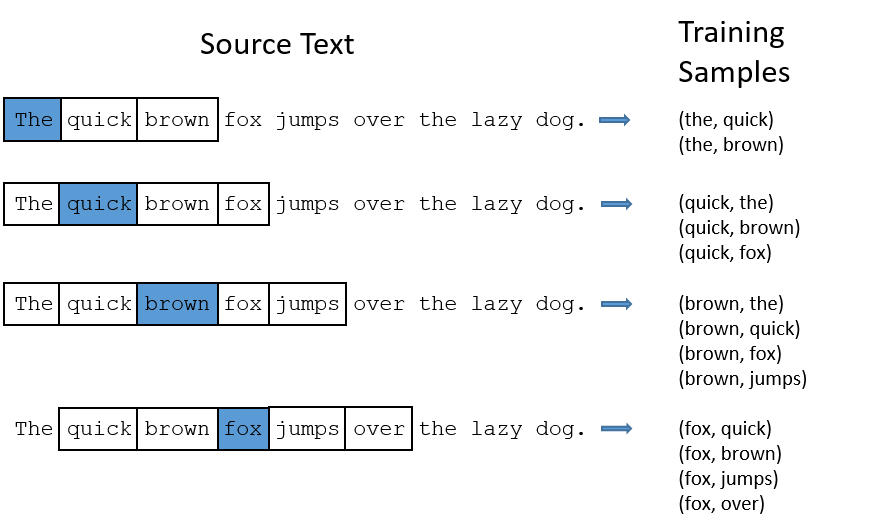
\includegraphics[scale = 0.45]{static/figures/skipgram_sample.png} 
\caption{Παράδειγμα δειγματοληψίας για την εκπαίδευση του μοντέλου \en{SkipGram} \cite{word2vec}}
\label{figure1.2}
\end{figure}

Οι λέξεις εισόδου αναπαριστώνται ως ένα διάνυσμα \(1 \times N\), όπου \(N\) το πλήθος των
λέξεων του λεξιλογίου. Το διάνυσμα αυτό έχει την τιμή ````1\'''' στη θέση που αντιστοιχεί στη 
λέξη εισόδου και ````0'''' αλλού. Η έξοδος του νευρωνικού είναι επίσης ένα \(1 \times N\)
διάνυσμα που σε κάθε θέση περιέχει την πιθανότητα να επιλέξουμε τυχαία τη λέξη στην οποία 
αντιστοιχεί η θέση αυτή. Στο παρακάτω Σχήμα (\ref{figure1.3}) φαίνεται η αρχιτεκτονική
του νευρωνικού, αν η λέξη εισόδου είναι ````\en{ants}'''' (μτφ. μυρμήγκια).

\begin{figure}[!ht] \centering
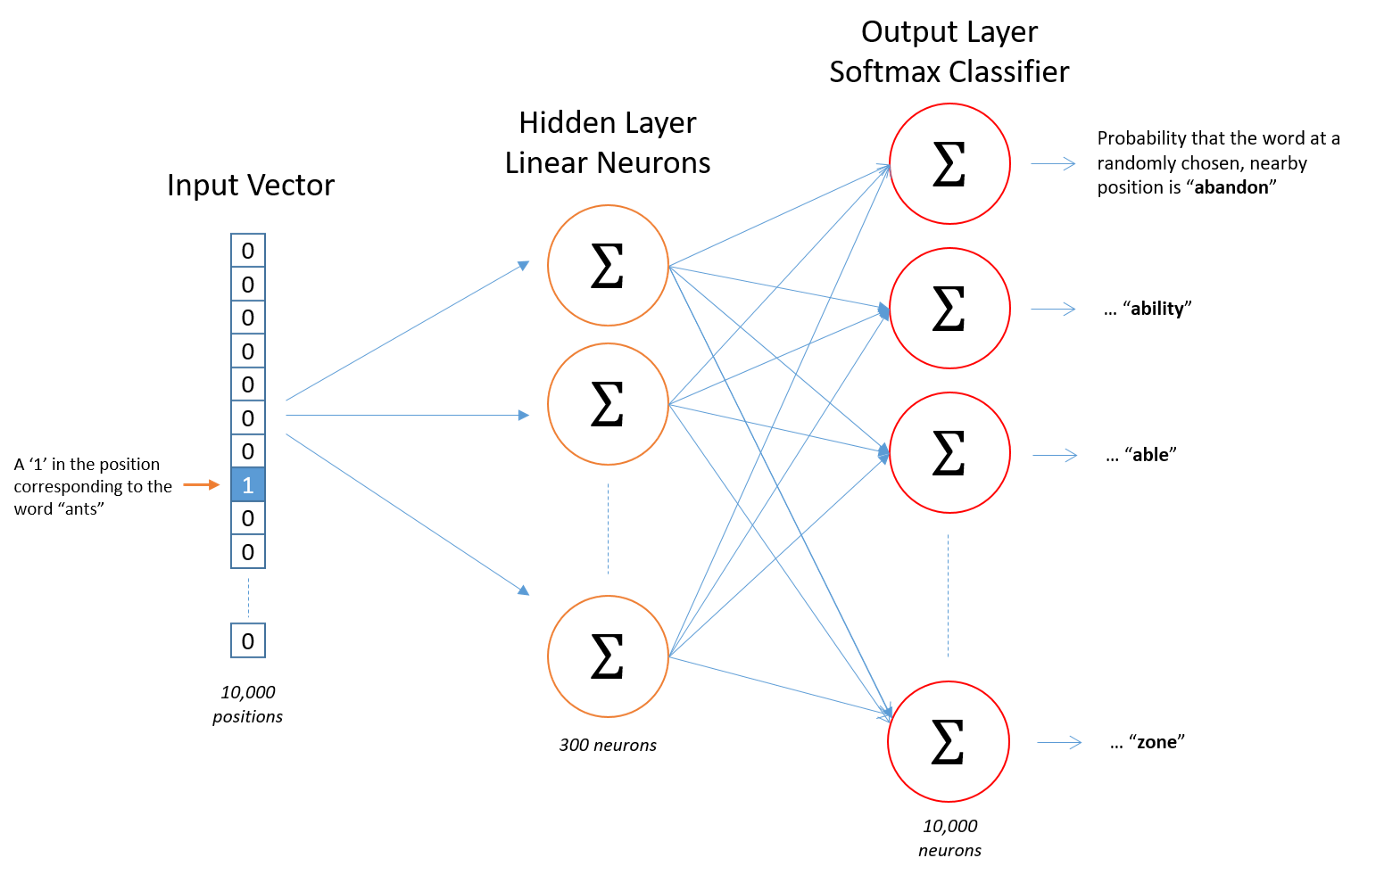
\includegraphics[scale = 0.3]{static/figures/skipgram_nn.png} 
\caption{Δομή του νευρωνικού του μοντέλου \en{SkipGram} \cite{word2vec}}
\label{figure1.3}
\end{figure}

Για το κρυφό στρώμα, δεν υπάρχει συνάρτηση ενεργοποίησης (\en{activation function}), ωστόσο 
στην έξοδο χρησιμοποιείται \en{softmax}. Υπενθυμίζεται ότι η συνάρτηση \en{softmax} είναι
μια συνάρτηση κανονικοποίησης, η οποία παίρνει σαν είσοδο ένα διάνυσμα \(1 \times K\) 
και το κανονικοποιεί σε μια κατανομή πιθανότητας \(K\) ενδεχομένων:

\begin{equation}
    \en{\sigma(\textbf{z})_i = \frac{e^{z_i}}{\sum_{j=1}^{K} e^{z_j}}}
\end{equation}

για \(i=1,\cdots,K\) και \(\textbf{z} = (z_1,\cdots,z_K) \in \mathbb{R}^K\)

Ουσιαστικά, η συνάρτηση \en{softmax} κανονικοποιεί τα στοιχεία του διανύσματος έτσι ώστε
να έχουν μοναδιαίο άθροισμα.

Έστω οτι επιλέχθηκε να αναπαραστήσουμε τις λέξεις με 300 διαστάσεις. Το κρυφό στρώμα
θα αναπαρασταθεί με έναν \(10000 \times 300\) πίνακα (10000 λέξεις στο λεξιλόγιο επί
300 διαστάσεις αναπαράστασης). Ο αριθμός διαστάσεων αναπαράστασης αποτελεί και αυτός
παράμετρο του μοντέλου. Στο τέλος, οι γραμμές του πίνακα αυτού θα είναι οι αναπαραστάσεις
των λέξεων. Στην περίπτωση των γράφων, το κρυφό στρώμα αναπαριστάται από έναν πίνακα
διαστάσεων \(N \times d\), όπου \(N\) το πλήθος των κόμβων του δικτύου και \(d\) ο αριθμός
διαστάσεων που έχει δοθεί σαν παράμετρος του αλγορίθμου. Η τεχνική \en{DeepWalk} 
χρησιμοποιεί αυτή τη λογική, ωστόσο η ακριβής λειτουργία της είναι παρόμοια με μια άλλη
τεχνική, τη \en{Node2Vec} \cite{node2vec}, η οποία εξηγείται σε επόμενη παράγραφο.


\subsection{Aναπαράσταση χωρίς τη χρήση τυχαίων περιπάτων}

Η εκμάθηση αναπαραστάσεων γράφων χωρίς τη χρήση τυχαίων περιπάτων βασίζεται στην εφαρμογή
τεχνικών βαθιάς μάθησης απευθείας στον γράφο ή στον πίνακα γειτνίασης ενός γράφου. Παρακάτω
αναφέρονται ονομαστικά κάποιες τεχνικές χωρίς επεξήγηση, μιας και κάτι τέτοιο ξεφεύγει από
τα πλαίσια της εργασίας.

\begin{itemize}
    \item \textbf{\en{Autoencoder}} (μτφ. Αυτοκωδικοποιητής): Κωδικοποιεί τον γράφο 
    σε ένα χώρο με τον κωδικοποιητή και τον αποκωδικοποιεί με τον αποκωδικοποιτή. Στόχος
    είναι η ελαχιστοποίηση του σφάλματος εισόδου-εξόδου \cite{pan2018adversarially}.
    \item \textbf{\en{Deep Neural Network}} (μτφ. Βαθύ Νευρωνικό Δίκτυο):  Χρησιμοποιεί \en{Convolutional Neural 
    Networks} (\en{CNN's}) (μτφ. Συνελικτικό Νευρωνικό Δίκτυο) για εκμάθηση
    αναπαραστάσεων από γράφους \cite{pmlr-v48-niepert16}.
\end{itemize}

\subsection{Από την αναπαράσταση κόμβων στην αναπαράσταση ακμών}

Το πρόβλημα της αναπαράστασης γράφων μπορεί, κατά περίπτωση, να οριστεί ως προς την είσοδο
και την έξοδο, με πολλούς τρόπους, ανάλογα με τις προϋποθέσεις της εκάστοτε τεχνικής που 
θα εφαρμοστεί, αλλά και ανάλογα με τον τύπο προβλήματος που πρόκειται να επιλύσουν
\cite{cai2017comprehensive}:

\begin{itemize}
    \item Είσοδος: \begin{itemize}
                        \item Ομογενής γράφος
                        \item Ετερογενής γράφος
                        \item Γράφος με χαρακτηριστικά κόμβων/ακμών
                        \item Γράφος κατασκευασμένος από μη-σχεσιακά δεδομένα
                   \end{itemize}
    \item Έξοδος: \begin{itemize}
                        \item Αναπαράσταση κόμβων
                        \item Αναπαράσταση ακμών
                        \item Υβριδική αναπαράσταση
                        \item Αναπαράσταση ολόκληρου γράφου
                  \end{itemize}
\end{itemize}

Για τους σκοπούς της εργασίας αυτής, για λόγους απλότητας, αποτελεσματικότητας και δυνατότητας 
βελτιστοποίησης επιλέχθηκε η χρήση αναπαράστασης κόμβων, και έπειτα κατασκευή της
αναπαράστασης ακμών από την αναπαράσταση κόμβων. Για την διεργασία αυτή, υπάρχουν διάφοροι
τελεστές \cite{node2vec}, οι οποίοι κατά περίπτωση διερευνώνται και επιλέγεται ο βέλτιστος για
τα εκάστοτε δεδομένα:

\begin{itemize}
    \item \en{Hadamard} : \begin{equation}
                            [f(u) \boxdot f(v)]_i = f_{i}(u) \ast f_{i}(v)
                          \end{equation} 
    \item \en{Average} : \begin{equation}
                            [f(u) \boxplus f(v)]_i = \frac{f_{i}(u) + f_{i}(v)}{2}   
                         \end{equation}
    \item \en{Weighted-L1} : \begin{equation}
                                \parallel f(u) \dot f(v) \parallel_{\Bar{1}_{i}} = 
                                |f_{i}(u) - f_{i}(v)|
                            \end{equation}
    \item \en{Weighted-L2} : \begin{equation}
                                \parallel f(u) \dot f(v) \parallel_{\Bar{2}_{i}} = 
                                |f_{i}(u) - f_{i}(v)|^2
                             \end{equation}
\end{itemize}

όπου \(f(u), f(v)\) η αναπαράσταση των κόμβων \(u, v\) αντίστοιχα και \(f_{i}(u)\) η 
\(i\)-οστή συνιστώσα της αναπαράστασης του κόμβου \(u\)


\subsection{Μηχανική μάθηση και ταξινόμηση}

Το πρόβλημα της ταξινόμησης είναι από τα πιο δημοφιλή για χρήση μηχανικής μάθησης. 
Ανήκει στην οικογένεια της επιβλεπόμενης (\en{supervised}) μηχανικής μάθησης, και στόχος
είναι η ανάπτυξη ενός μοντέλου που θα κατηγοριοποιεί ορθά τα δεδομένα εισόδου σε
μια σειρά κλάσεων. Το μοντέλο δηλαδή παίρνει σαν είσοδο μια παρατήρηση και στην έξοδο
βγάζει την κατηγορία στην οποία εμπίπτει αυτή η παρατήρηση. Η έξοδος δηλαδή είναι διακριτή
τιμή. Μια παραλλαγή του προβλήματος αποτελεί η Παλινδρόμηση (\en{Regression})
όπου η έξοδος είναι μια συνεχής τιμή, συνήθως μια πιθανότητα η είσοδος να εμπίπτει σε μια 
συγκεκριμένη κλάση. Θέτοντας ένα όριο π.χ. 0,5 στην έξοδο, οι τεχνικές παλινδρόμησης
χρησιμοποιούνται για προβλήματα ταξινόμησης. Για όριο (\en{Threshold}) ίσο με 0,5 
θεωρείται ότι άν η έξοδος δώσει μια πιθανότητα άνω από 0,5 μια παρατήρηση \(x\) 
να ανήκει στην κλάση \(y\), τότε η παρατήρηση ανήκει στην κλάση αυτή, και ούτω καθεξής (κ.ο.κ.).

Ένα πρόβλημα δυαδικής ταξινόμησης ή παλινδρόμησης είναι ένα πρόβλημα στο οποίο υπάρχουν 
2 δυνατές κλάσεις. Στα πλαίσια της εργασίας θα χρησιμοποιηθεί μια τεχνική παλινδρόμησης,
η \en{Logistic Regression with Cross-Validation} (μτφ. Λογιστική Παλινδόμηση με διασταυρωμένη επικύρωση) για την ανάπτυξη ενός μοντέλου Ταξινόμησης.

\subsubsection{Λογιστική παλινδρόμηση}

Το λογιστικό μοντέλο χρησιμοποιείται για να μοντελοποιήσει την πιθανότητα εμφάνισης ενός
γεγονότος δυαδικής φύσεως, όπως είναι η νίκη/ήττα, επιτυχία/αποτυχία κ.ο.κ. Οι πιθανές
 εκβάσεις μπορούν να είναι και περισσότερες από 2, ωστόσο το μοντέλο δίνει μια πιθανότητα
(από 0 ως 1) κάποια παρατήρηση να εμπίπτει σε κάθε κλάση, και οι πιθανότητες κάθε κλάσης
για κάθε παρατήρηση έχουν μοναδιαίο άθροισμα.

Η λογιστική παλινδρόμηση \cite{10.1001/jama.2016.7653} αποτελεί ένα στατιστικό μοντέλο που
στη βασική του μορφή υλοποιεί την προαναφερθείσα λειτουργία. Από μαθηματικής άποψης, το 
λογιστικό μοντέλο έχει μια εξαρτημένη μεταβλητή με δύο πιθανές τιμές που ανήκουν στο δισύνολο \(\{0, 1\}\).
Ο λογάριθμος της πιθανότητας της τιμής ````1'''' είναι ένας γραμμικός (ή μη) συνδυασμός ενός
αριθμού ανεξάρτητων μεταβλητών που ονομάζονται μεταβλητές πρόβλεψης (\en{predictors}). Οι
ανεξάρτητες μεταβλητές μπορούν να είναι είτε δυαδικές είτε συνεχείς. Η τελική πιθανότητα της
τιμής ````1'''' μπορεί να είναι από 0 (σίγουρα η τιμή ````0'''') μέχρι και 1 (σίγουρα η τιμή ````1''''). Η
συνάρτηση που μετατρέπει το λογάριθμο σε πιθανότητα είναι η λογιστική συνάρτηση
(\ref{logistic_func}), αλλά χρησιμοποιούνται και μοντέλα με διαφορετικές σιγμοειδείς
συναρτήσεις. Το κύριο χαρακτηριστικό των λογιστικών μοντέλων είναι πως η αύξηση μίας
ανεξάρτητης μεταβλητής επηρεάζει την τελική πιθανότητα κατά σταθερό ρυθμό, και κάθε 
ανεξάρτητη μεταβλητή έχει την δική της παράμετρο.

\begin{equation}
    S(x) = \frac{1}{1 + e^{-x}} = \frac{e^x}{e^{x} + 1}
    \label{logistic_func}
\end{equation}

\begin{figure}[!ht] \centering
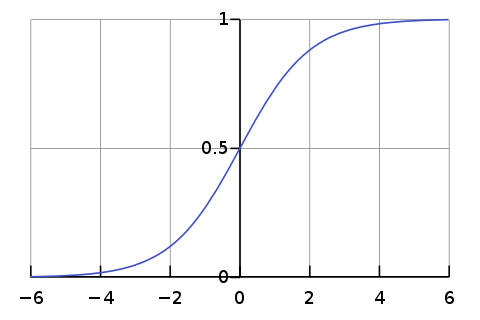
\includegraphics[scale = 0.6]{static/figures/logistic_curve.png} 
\caption{Τυπική μορφή λογιστικής συνάρτησης \cite{10.1001/jama.2016.7653}}
\label{figure1.4}
\end{figure}

Στην περίπτωση του δυαδικού μοντέλου λογιστικής παλινδρόμησης, η εξαρτημένη μεταβλητή είναι
κατηγορική, δηλαδή όπως προαναφέρθηκε έχει δύο πιθανές τιμές, που αναφέρονται και ως κλάσεις.
Το λογιστικό μοντέλο ωστόσο απλώς δίνει μια πιθανότητα σε κάθε μία από τις δύο πιθανές
κλάσεις και από μόνο του δεν αποτελεί ταξινομητή. Για να χρησιμοποιηθεί σαν ταξινομητής
συνήθως επιλέγεται όπως αναφέραμε ένα κατώφλι (\en{threshold}). Οι συντελεστές του μοντέλου
δεν υπολογίζονται με κάποια συγκεκριμένη μεθοδολογία, και για το λόγο αυτό στα πλαίσια της
εργασίας χρησιμοποιήθηκε η τεχνική της διασταυρωμένης επικύρωσης (\en{Cross Validation}).
Η τεχνική αυτή καθιστά δυνατή την αυτόματη βελτιστοποίηση των παραμέτρων του μοντέλου.
Ο τρόπος λειτουργίας της τεχνική αυτής ξεφεύγει από τα πλαίσια της εργασίας αυτής.

\subsection{Επικύρωση μοντέλων μηχανικής μάθησης}

Για την ορθή ανάπτυξη μοντέλων με χρήση μηχανικής μάθησης, είναι απαραίτητη η χρήση κάποιων
μετρικών για την διαπίστωση της αποτελεσματικότητας του μοντέλου υπο ανάπτυξη. Οι μετρικές
αφορούν την περίπτωση της επιβλεπόμενης μηχανικής μάθησης, όπου οι ορθές τιμές εξόδου 
κατά το στάδιο της εκπαίδευσης είναι γνωστές. Συνήθως χρησιμοποιείται μια συνάρτηση που 
συγκρίνει τις εξόδους του μοντέλου με τις ορθές τιμές και δίνει κάποια τιμή που όσο 
μεγαλύτερη είναι τόσο πιο ακριβές είναι το μοντέλο. 

Για την περίπτωση των ταξινομητών και ειδικότερα της δυαδικής ταξινόμησης για την έξοδο
του μοντέλου υπάρχουν οι εξής περιπτώσεις σχετικά με την ορθότητα του αποτελέσματος για
μία παρατήρηση:

\begin{itemize}
    \item Αληθές Θετικό (\en{True Positive - TP}): Ο ταξινομητής κατέταξε την παρατήρηση
    στην κλάση ````1'''' ορθά, δηλαδή η παρατήρηση όντως ανήκει στην κλάση ````1''''
    \item Ψευδές Θετικό (\en{False Positive - FP}): Ο ταξινομητής κατέταξε την παρατήρηση
    στην κλάση ````1'''' λανθασμένα, δηλαδή η παρατήρηση ανήκει στην κλάση ````0''''
    \item Αληθές Αρνητικό (\en{True Negative - TN}): Ο ταξινομητής κατέταξε την παρατήρηση
    στην κλάση ````0'''' ορθά, δηλαδή η παρατήρηση όντως ανήκει στην κλάση ````0''''
    \item Ψευδές Αρνητικό (\en{False Negative - FN}): Ο ταξινομητής κατέταξε την παρατήρηση
    στην κλάση ````0'''' λανθασμένα, δηλαδή η παρατήρηση ανήκει στην κλάση ````1''''
\end{itemize}

Από τα παραπάνω σχηματίζεται ο \en{Confusion Matrix} (μτφ. Πίνακας Σύγχυσης) που στην περίπτωση
της δυαδικής ταξινόμησης είναι ένας \(2 \times 2\) πίνακας. Στην εικόνα \ref{figure1.5} 
δίνεται ένα παράδειγμα όπου οι κλάσεις αντί για ````0'''' και ````1'''' είναι ````\en{Yes}'''' και ````\en{No}''''.

\begin{figure}[!ht] \centering
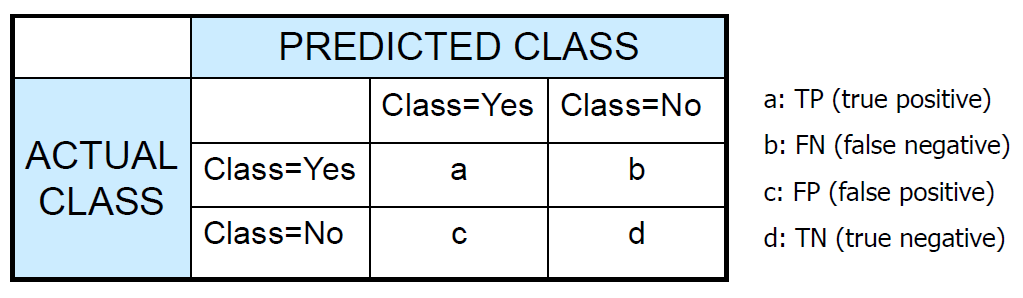
\includegraphics[scale = 0.6]{static/figures/conf_matrix.png} 
\caption{Τυπική μορφή πίνακα σύγχυσης \cite{DataMining}}
\label{figure1.5}
\end{figure}

Επίσης σχηματίζεται και η μετρική (\en{Accuracy}) (μτφ. Ακρίβειας), που δίνει το ποσοστό των
ορθά ταξινομημένων παρατηρήσεων σε σχέση με το πλήθων των ταξινομήσεων:

\begin{equation}
    Accuracy = \frac{TP + TN}{TP + TN + FP + FN}
\end{equation}

Η μετρική \en{Accuracy}, ενώ είναι πολύ δημοφιλής, υπάρχουν περιπτώσεις στις οποίες δίνει λανθασμένη εικόνα για την
ποιότητα του μοντέλου. Για παράδειγμα για ένα σύνολο παρατηρήσεων που έχει 9990 εγγραφές
που ανήκουν στην κλάση ````0'''' και 10 εγγραφές που ανήκουν στην κλάση ````1'''', αν το μοντέλο 
ταξινομήσει όλες τις παρατηρήσεις στην κλάση ````0'''' δίνεται μια τιμή \en{Accuracy} = \(99.9\%\),
που ενώ είναι μια πολύ καλή τιμή ακρίβειας, το μοντέλο υπό ανάπτυξη είναι πολύ κακό.

Υπάρχουν και μερικές μετρικές πολωμένες ως προς μια κατηγορία αποτελεσμάτων. Για παράδειγμα,
η μετρική \en{Precision} (μτφ. Ευστοχίας), είναι πολωμένη ως προς τα \en{TP,
FP}:

\begin{equation}
    Precision = \frac{TP}{TP + FP}
\end{equation}

H μετρική \en{Recall} (μτφ. Ανάκλησης), είναι πολωμένη ως προς τα \en{TP, FN}:

\begin{equation}
    Recall = \frac{TP}{TP + FN}
\end{equation}

Από τις δύο τελευταίες μετρικές προκύπτει η μετρική ````\en{F1-Score}'''' που τις συνδυάζει 
ως τον αρμονικό μέσο, και όχι τον αριθμητικό. Επιλέγεται ο αρμονικός μέσος επειδή ````τιμωρεί''''
περισσότερο τις ακραίες περιπτώσεις. Για παράδειγμα, σε έναν ταξινομητή με εντελώς τυχαία
πρόβλεψη θα δίνει μια ακρίβεια περίπου \(50\%\). Για τις ανάγκες του παραδείγματος θεωρείται
πως η τιμή της \en{Recall} = 0 και \en{Precision} = 1. Αν επιλεγόταν ο αριθμητικός μέσος
θα εδίνε μια τιμή 0.5. Ο αρμονικός μέσος δίνει μια τιμή 0, που αντιπροσωπεύει καλύτερα την
αποτελεσματικότητα του μοντέλου που είναι μηδαμινή, αφού ουσιαστικά αγνοεί την είσοδο και
````προβλέπει'''' τυχαία. Η τιμή της μετρικής δίνεται από τον τύπο:

\begin{equation}
    F1\_Score = 2 * \frac{Recall * Precision}{Precision + Recall}
\end{equation}

Μια ακόμα εξαιρετικά δημοφιλής είναι οι καμπύλες \en{Receiver Operating
Characteristics (ROC)} (μτφ. Χαρακτηριστικά Λειτουργίας Δέκτη). Εμφανίστηκαν τη δεκαετία του
1950 στο πεδίο της ανάλυσης σημάτων για την ανάλυση θορυβοδών σημάτων \cite{DataMining}. 

\subsubsection{Καμπύλες \en{ROC}}

Οι καμπύλες \en{ROC} αναπαριστούν τις \en{TP} παρατηρήσεις στον άξονα \en{y} ως προς τις
\en{FP} παρατηρήσεις, στον άξονα \en{x}. Η επίδοση ενός μοντέλου ταξινόμησης αναπαρίσταται 
ως ένα σημείο στην καμπύλη. Αλλάζοντας το κατώφλι του αλγορίθμου, αλλάζει και η θέση του
σημείου. Το σημείο [0,0] αντιπροσωπεύει τιμή κατωφλίου 1, δηλαδή όλες οι παρατηρήσεις
ταξινομούνται στην κλάση ````0'''', ενώ το [1,1] το αντίστροφο, δηλαδή όλες οι παρατηρήσεις
ταξινομούνται στην κλάση ````1''''. Το σημείο [0,1] είναι το ιδανικό, που αντιπροσωπεύει την
περίπτωση όπου όλες οι παρατηρήσεις ταξινομήθηκαν σωστά, ενώ η κύρια διαγώνιος αντιπροσωπεύει
έναν τυχαίο ταξινομητή. Αν τα σημεία της καμπύλης είναι κάτω από την κύρια διαγώνιο, 
τότε ο ταξινομητής ταξινομεί τις παρατηρήσεις ανάποδα. Τέλος, η μετρική \en{Area Under Curve Score (AUC-Score)} (μτφ. Μετρική Περιοχής Κάτω από την Καμπύλη)
δίνει το ποσοστό της επιφάνειας που βρίσκεται κάτω από την καμπύλη 
ως προς την συνολική επιφάνεια. Στην \ref{figure1.6} δίνεται ένα παράδειγμα καμπύλης 
\en{ROC}.

\begin{figure}[!ht] \centering
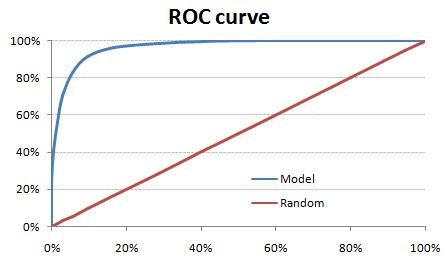
\includegraphics[scale = 1]{static/figures/ROC.jpg} 
\caption{Ενδεικτική μορφή καμπύλης \en{ROC} \cite{DataMining}}
\label{figure1.6}
\end{figure}


\section{Τεχνικές εξαγωγής αναπαραστάσεων}

Όπως έχει γίνει ήδη αντιληπτο, για να χρησιμοποιηθεί μηχανική μάθηση σε ένα πρόβλημα με
δεδομένα σε μορφή γράφου θα πρέπει πρώτα ο τελευταίος να μετατραπεί σε μια πιο παραδοσιακή
μορφή συνόλου δεδομένων, αυτή που αντιπροσωπεύει ένα σύνολο παρατηρήσεων/σημείων. Για τον
σκοπό αυτό έχουν αναπτυχθεί πολλές τεχνικές, ωστόσο στην εργασία αυτή επιλέχθηκαν και
χρησιμοποιήθηκαν 3 συγκεκριμένες οι οποίες θα αναλυθούν στη συνέχεια. Και οι τρείς τεχνικές
χρησιμοποιούν τεχνικές μη-επιβλεπόμενης μηχανικής μάθησης.

\subsection{\en{Node2Vec}} \label{n2v}

Η πρώτη τεχνική εξαγωγής αναπαραστάσεων κόμβων \en{node features}) από γράφο που επιλέχθηκε
είναι η \en{Node2Vec} \cite{node2vec}. Η βασική ιδέα που υλοποιεί αυτή η τεχνική είναι η
εξής: κόμβοι που βρίσκονται ````κοντά'''' σε ένα γράφο αναπαριστώνται με n-διάστατα σημεία στο
n-διάστατο χώρο που θα είναι εξ' ίσου ````κοντά''''. Διατηρείται δηλαδή η ιδιότητα των γειτονικών
σημείων κατά τη μετάβαση από τη μια μορφή αναπαράστασης των δεδομένων (γράφος) στην άλλη
(σημεία στο χώρο). Η τεχνική αυτή αποτελεί εξέλιξη μιας προϋπάρχουσας τεχνικής, της
\en{DeepWalk} \cite{DeepWalk}.

Η \en{Node2Vec} αρχικά δειγματοληπτεί τον γράφο πραγματοποιώντας ````τυχαίους περιπάτους'''' πάνω
σε αυτόν. Ξεκινώντας από ένα τυχαίο κόμβο, έστω \(u_i\), διασχίζει τον γράφο από κόμβο σε κόμβο με
τυχαία σειρά, σχηματίζοντας ένα μονοπάτι συγκεκριμένου μήκους \(l\), το οποίο αποτελεί το
δείγμα. Το αποτέλεσμα είναι μια αλληλουχία κόμβων \({u_1, u_2,...,u_k}\). Αυτή η διαδικασία
επαναλαμβάνεται \(k\) φορές για κάθε κόμβο. Η σημασία του \(l\) και του \(k\) είναι πολύ
υψηλή. Όσο αυξάνεται το \(k\), τόσο περισσότερο εξερευνάται ο γράφος, και τόσο περισσότερα
μονοπάτια δημιουργούνται. Όσο αυξάνεται το \(l\), τόσο αυξάνει το μήκος κάθε περιπάτου, και
άρα όλο και πιο μακρινοί κόμβοι λαμβάνονται υπόψιν ως ````γειτονικοί''''. Στη συνέχεια, το δείγμα
δίνεται ως είσοδος σε ένα μοντέλο \en{SkipGram} (Παράγραφος \ref{SkipGram}).

\subsubsection{Παράμετροι \en{Node2Vec}}

Ο \en{Node2Vec} δειγματοληπτεί τον γράφο όπως προαναφέραμε, και επιστρέφει έναν πίνακα 
\(N \times d\), όπου η κάθε γραμμή αντιστοιχεί σε κάθε κόμβο του δικτύου. Για να το πετύχει
αυτό δέχεται κάποιες παραμέτρους:

\begin{itemize}
    \item Αριθμός περιπάτων από κάθε κόμβο
    \item Μήκος κάθε περιπάτου
    \item \en{Q}, όπου \(1/Q\) η πιθανότητα κατά τον περίπατο να μεταπηδήσει 
    από έναν κόμβο \(u_i\) σε έναν γειτονικό κόμβο \(u_j\)
    \item \en{P}, όπου \(1/P\) η πιθανότητα κατά τον περίπατο να μεταπηδήσει 
    από έναν κόμβο \(u_i\) στον ίδιο κόμβο \(u_i\)
\end{itemize}

Επί της ουσίας, οι παράμετροι \(Q,P\) ρυθμίζουν την εστίαση του αλγορίθμου στην διατήρηση
των τοπικών γειτονιών ή της γενικότερης δομής του γράφου. Τέλος, τα βάρη των ακμών
λαμβάνονται υπ' όψιν, οπότε η τελική πιθανότητα μετάβασης για κάθε κόμβο είναι συνάρτηση των
3 παραμέτρων (\(Q,P,w\)). Το Σχήμα \ref{figure1.7} απεικονίζει ένα παράδειγμα λειτουργίας
του \en{Node2Vec} για \(d = 2\).

\begin{figure}[!ht] \centering
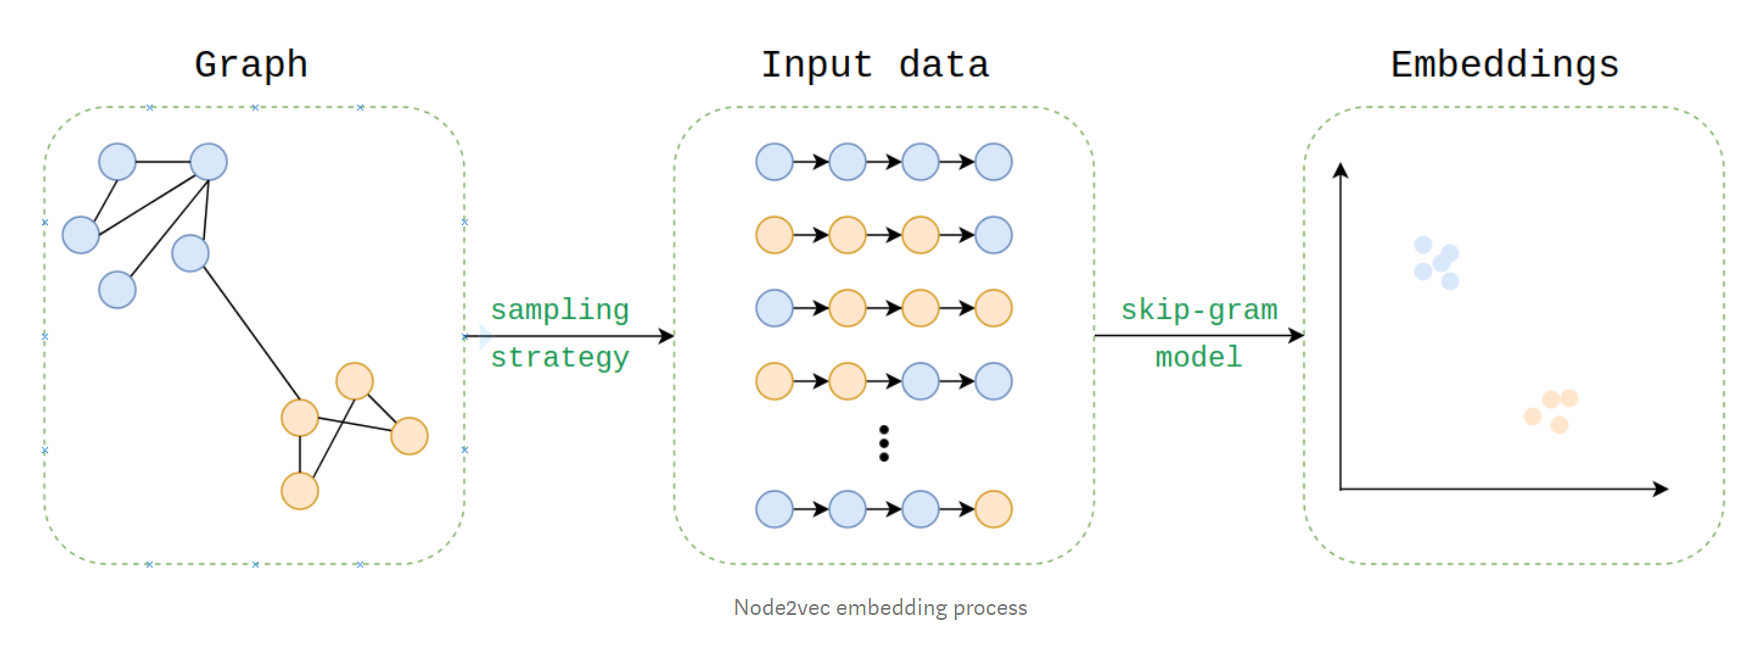
\includegraphics[scale = 0.3]{static/figures/n2v_figure.png} 
\caption{Τρόπος λειτουργίας \en{Node2Vec} για \(d = 2\) \cite{Node2VecImpl}}
\label{figure1.7}
\end{figure}

\subsection{\en{CTDNE}} \label{CTDNE}

Η δεύτερη τεχνική εξαγωγής αναπαραστάσεων είναι η \en{CTDNE - Continuous-Time Dynamic
Network Embeddings} \cite{CTDNE}. Η τεχνική αυτή ενσωματώνει τη χρονική παράμετρο στο
πρόβλημα εξαγωγής αναπαραστάσεων γράφου. Αφορά γράφους που αντιπροσωπεύουν ένα πρόβλημα
παραμετροποιημένο ως προς τον χρόνο. Πρακτικά στις περισσότερες εφαρμογές αυτό υλοποιείται
με τα βάρη των ακμών, όπου το βάρος μιας ακμής εμπεριέχει την πληροφορία για το πότε
δημιουργήθηκε.

Η \en{CTDNE} έχει παρόμοια λειτουργία με την \en{Node2Vec}, ωστόσο διαφέρει στον τρόπο
δειγματοληψίας τυχαίων περιπάτων. Εισάγει την έννοια των χρονικών τυχαίων περίπατων 
\({u_1, u_2,\cdots,u_k}\), όπου \(T(u_i,u_{i+1}) \leq T(u_{i+1},u_{i+2})\), δηλαδή η χρονική
στιγμή που δημιουργήθηκε η ακμή μεταξύ των κόμβων (\(u_i,u_{i+1}\)) είναι πρεσβύτερη από τη
χρονική στιγμή που δημιουργήθηκε η ακμή μεταξύ των κόμβων (\(u_{i+1},u_{i+2}\)). 
Οι δημιουργοί της τεχνικής δίνουν 3 επιλογές ως προς το όσο πολωμένη θα είναι η επιλογή
αρχικών ακμών ως προς τον χρόνο(\(Pr(e)\) η πιθανότητα να επιλεγεί η ακμή \(e\)):

\begin{itemize}
    \item Μη πολωμένη, όπου \(Pr(e) = 1/|E_T|\)
    \item Πολωμένη\begin{itemize}
            \item Εκθετικά, όπου 
            
            \begin{equation}
                Pr(e) = \frac{exp[T(e) - t_{min}]}
                {\sum_{e^{'} \in E_T} exp[T(e^{'}) - t_{min}]}
            \end{equation}
            
            και \(t_{min}\) η παλαιότερη χρονική στιγμή που υπάρχει στον γράφο. 
            Αυτή η κατανομή είναι σημαντικά πολωμένη ως προς τις νεότερες ακμές
            
            \item Γραμμικά, όπου
            
            \begin{equation}
                Pr(e) = \frac{\eta(e)}{\sum_{e^{'} \in E_T} \eta(e^{'})}
            \end{equation}
            
            και \(\eta(e)\) μια συνάρτηση που συσχετίζει κάθε ακμή με ένα δείκτη, και η
            παλαιότερη ακμή όλων έχει \(\eta(e) = 1\)
            
        \end{itemize}
\end{itemize}

Λόγω της φύσης του αλγορίθμου, είναι βέλτιστο να διατυπωθούν οι παράμετροι που δέχεται ο
αλγόριθμος ως εξής:

\begin{itemize}
    \item Αριθμός περιπάτων από κάθε κόμβο (\(R\))
    \item Μήκος κάθε περιπάτου (\(L\))
    \item Παράθυρο περιβάλλοντος (\en{Context Window}, \(\omega\))
    \item Αριθμός παραθύρων περιβάλλοντος (\(\beta\))
    \item Τρόπος επιλογής ακμής (Πολωμένη Εκθετικά/Γραμμικά, Μη Πολωμένη)
\end{itemize}

Σε αντίθεση με τη \en{Node2Vec}, δεν είναι χρήσιμο να ορίσουμε ένα μήκος περιπάτου, αλλά ένα
εύρος αποδεκτών μηκών μονοπατιού, αφού στην τεχνική αυτή δίνεται βάρος στην χρονική
εγκυρότητα του μονοπατιού. Ειδικότερα για την παράμετρο \(\beta\), σύμφωνα με το
\cite{CTDNE} ορίζεται ως συνάρτηση των άλλων παραμέτρων:
\begin{equation} \label{2.19}
    \beta = R \times N \times ( L - \omega + 1)
\end{equation}
όπου \(N\) ο αριθμός των κόμβων του γράφου.

\subsection{\en{GraphSAGE}} \label{gsage}

Η τρίτη τεχνική εξαγωγής αναπαραστάσεων που επιλέχθηκε είναι η \en{GraphSage}
\cite{GraphSAGE}. Η ειδοποιός διαφορά ανάμεσα σε αυτή και στις προηγούμενες
είναι ότι η \en{GraphSage} χρησιμοποιεί τα χαρακτηριστικά των κόμβων (\en{node attributes})
για να παράξει αναπαραστάσεις αυτών (\en{node embeddings}).

Οι προηγούμενες τεχνικές αποτελούν μεταγωγικές (\en{transductive}) μεθόδους, δηλαδή εξάγουν
αναπαραστάσεις από ένα δεδομένο και σταθερό γράφο. Η \en{GraphSage} αποτελεί μια επαγωγική
(\en{inductive}) μέθοδο εξαγωγής αναπαραστάσεων, που σημαίνει ότι λειτουργεί και σε δυναμικά
περιβάλλοντα, παράγοντας αναπαραστάσεις για νέους κόμβους χωρίς την ανάγκη επανεκπαίδευσης
του συστήματος. Αυτό πετυχαίνεται με τη χρήση συναθροιστικών συναρτήσεων 
(\en{aggregator functions}), των οποίων ο ρόλος είναι να συναθροίζουν πληροφορία για κάθε
κόμβο από τους γείτονές τους. Τα βάρη των συναθροιστικών συναρτήσεων μπορεί να είναι 
σταθερά ή να προκύπτουν μέσα από εκπαίδευση, ανάλογα με την συνάρτηση.

Για την εξαγωγή αναπαραστάσεων με συναθροιστικές συναρτήσεις, αρχικά παράγονται
αναπαραστάσεις για κάθε κόμβο από τα χαρακτηριστικά του. Έπειτα, για κάθε κόμβο, παράγεται
μια αναπαράσταση αυτού βάσει της ````γειτονιάς'''' του, δηλαδή όσων κόμβων έχουν απόσταση \(K\)
από αυτόν \(K \in [1,n)\) και συνενώνεται με την υπάρχουσα αναπαράσταση για τον κόμβο αυτό.
Τέλος το συνολικό διάνυσμα της αναπαράστασης μπαίνει σαν είσοδο σε ένα νευρωνικό δίκτυο,
ώστε να ανανεωθεί η τελική αναπαράσταση του κόμβου. Αφού η διαδικασία επαναληφθεί για κάθε
κόμβο, κανονικοποιούνται οι αναπαραστάσεις ώστε να έχουν μοναδιαίο άθροισμα.
Παρουσιάζεται στο Σχήμα \ref{figure1.8} ο αλγόριθμος σε ψευδοκώδικα όπως δίνεται στο
\cite{GraphSAGE}.

\begin{figure}[!ht] \centering
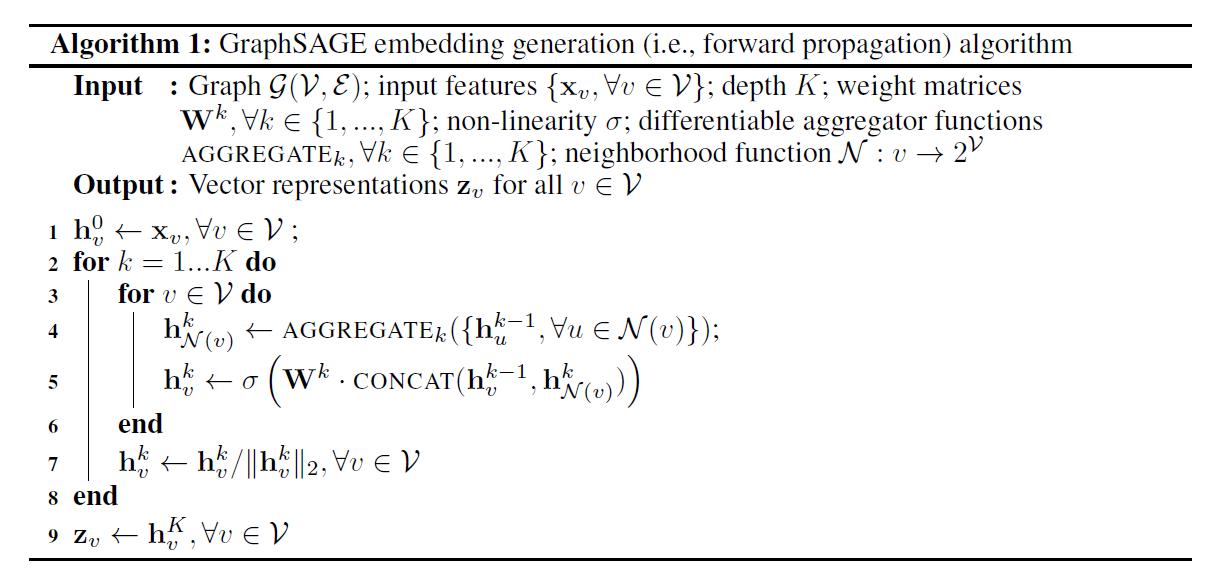
\includegraphics[scale = 0.5]{static/figures/GSAGE_algo.png} 
\caption{Αλγόριθμος  \en{GraphSage} παραγωγής  αναπαραστάσεων κόμβων \cite{GraphSAGE}}
\label{figure1.8}
\end{figure}

Για την βελτιστοποίηση των βαρών των συναρτήσεων συνάθροισης χρειαζόμαστε μια συνάρτηση
απώλειας (\en{loss function}), η οποία να ικανοποιεί τον περιορισμό οτι γειτονικοί κόμβοι
θα πρέπει να έχουν παρόμοιες αναπαραστάσεις και απομακρυσμένοι κόμβοι να έχουν
αρκετά διαφορετικές αναπαραστάσεις. Η συνάρτηση που προτείνεται στο
\cite{GraphSAGE} είναι η:

\begin{equation}
    J_{G}(\boldsymbol{z}_{u}) = -\log(\sigma)(\boldsymbol{z}_{u}^{T}\boldsymbol{z}_{v})
    - Q \cdot E_{u_{n}~P_{n}(v)} \log(\sigma(-\boldsymbol{z}_{u}^{T}\boldsymbol{z}_{v_{n}}))
\end{equation}

όπου \(u\) και \(v\) είναι 2 γειτονικοί κόμβοι και η συνάρτηση υπολογίζεται ως προς \(u\).
Ο πρώτος όρος μεγιστοποιεί την ομοιότητα των αναπαραστάσεων των \(u\) και \(v\). Στον δεύτερο
ο όρος \(Q\) είναι ο αριθμός των αρνητικών δειγμάτων (μη γειτονικοί κόμβοι) και \(v_n\) 
ένα αρνητικό δείγμα από μια κατανομή αρνητικών δειγμάτων. Οπότε ο δεύτερος όρος μεγιστοποιεί
τη διαφοροποίηση των μη-γειτονικών κόμβων και \(\sigma\) η σιγμοειδής συνάρτηση. Τέλος,
επισημαίνεται ότι η συνάρτηση αυτή υλοποιεί μια μη-επιβλεπόμενη μέθοδο εκμάθησης,
ωστόσο είναι δυνατό ο χρήστης να υλοποιήσει τον αλγόριθμο σε πλαίσιο επιβλεπόμενης 
εκπαίδευσης.